\documentclass[11pt]{article}
\usepackage[top=1cm, bottom=2cm, left=1cm, right=1cm]{geometry}
\usepackage{ctex}
\usepackage{algorithm}
\usepackage{algorithmicx}
\usepackage{algpseudocode}
\usepackage{amsthm,amsmath,amssymb}
\usepackage[colorlinks=true,linkcolor=blue]{hyperref}
\usepackage{listings}
\usepackage{xcolor,xparse}
\usepackage{realboxes}
\usepackage{graphics}
\usepackage{graphicx}
\usepackage{mathrsfs}
\usepackage{wrapfig}
\usepackage{subfigure}
\usepackage{pifont}

\definecolor{cmdbg}{rgb}{0.9,0.9,0.9}
\lstset{%
	basicstyle=\ttfamily,
	breaklines = true,
	backgroundcolor=\color{cmdbg},
}
\DeclareDocumentCommand{\ccmd}{v}{% 参数 v 表示工作方法类似于 \verb
    \Colorbox{cmdbg}{\csname lstinline\endcsname!#1!}%
}

\makeatletter
\newenvironment{breakablealgorithm}
  {% \begin{breakablealgorithm}
   \begin{center}
     \refstepcounter{algorithm}% New algorithm
     \hrule height.8pt depth0pt \kern2pt% \@fs@pre for \@fs@ruled
     \renewcommand{\caption}[2][\relax]{% Make a new \caption
       {\raggedright\textbf{\ALG@name~\thealgorithm} ##2\par}%
       \ifx\relax##1\relax % #1 is \relax
         \addcontentsline{loa}{algorithm}{\protect\numberline{\thealgorithm}##2}%
       \else % #1 is not \relax
         \addcontentsline{loa}{algorithm}{\protect\numberline{\thealgorithm}##1}%
       \fi
       \kern2pt\hrule\kern2pt
     }
  }{% \end{breakablealgorithm}
     \kern2pt\hrule\relax% \@fs@post for \@fs@ruled
   \end{center}
  }
\makeatother

\author{谢昀城 22307110070}
\title{计算物理作业2}

\begin{document}
\maketitle


\section{题目1:求方程的根}
\subsection{题目描述}
Sketch the function$x^3-5x+3=0$
\begin{enumerate}
    \item Determine the two positive roots to 4 decimal places using the bisection method. Note: You first need to bracket each of the roots.
    \item Take the two roots that you found in the previous question (accurate to 4 decimal places) and “polish them up” to 14 decimal places using the Newton-Raphson method.
    \item Determine the two positive roots to 14 decimal places using the hybrid method.
\end{enumerate}
\begin{figure}[htpb]
    \centering
    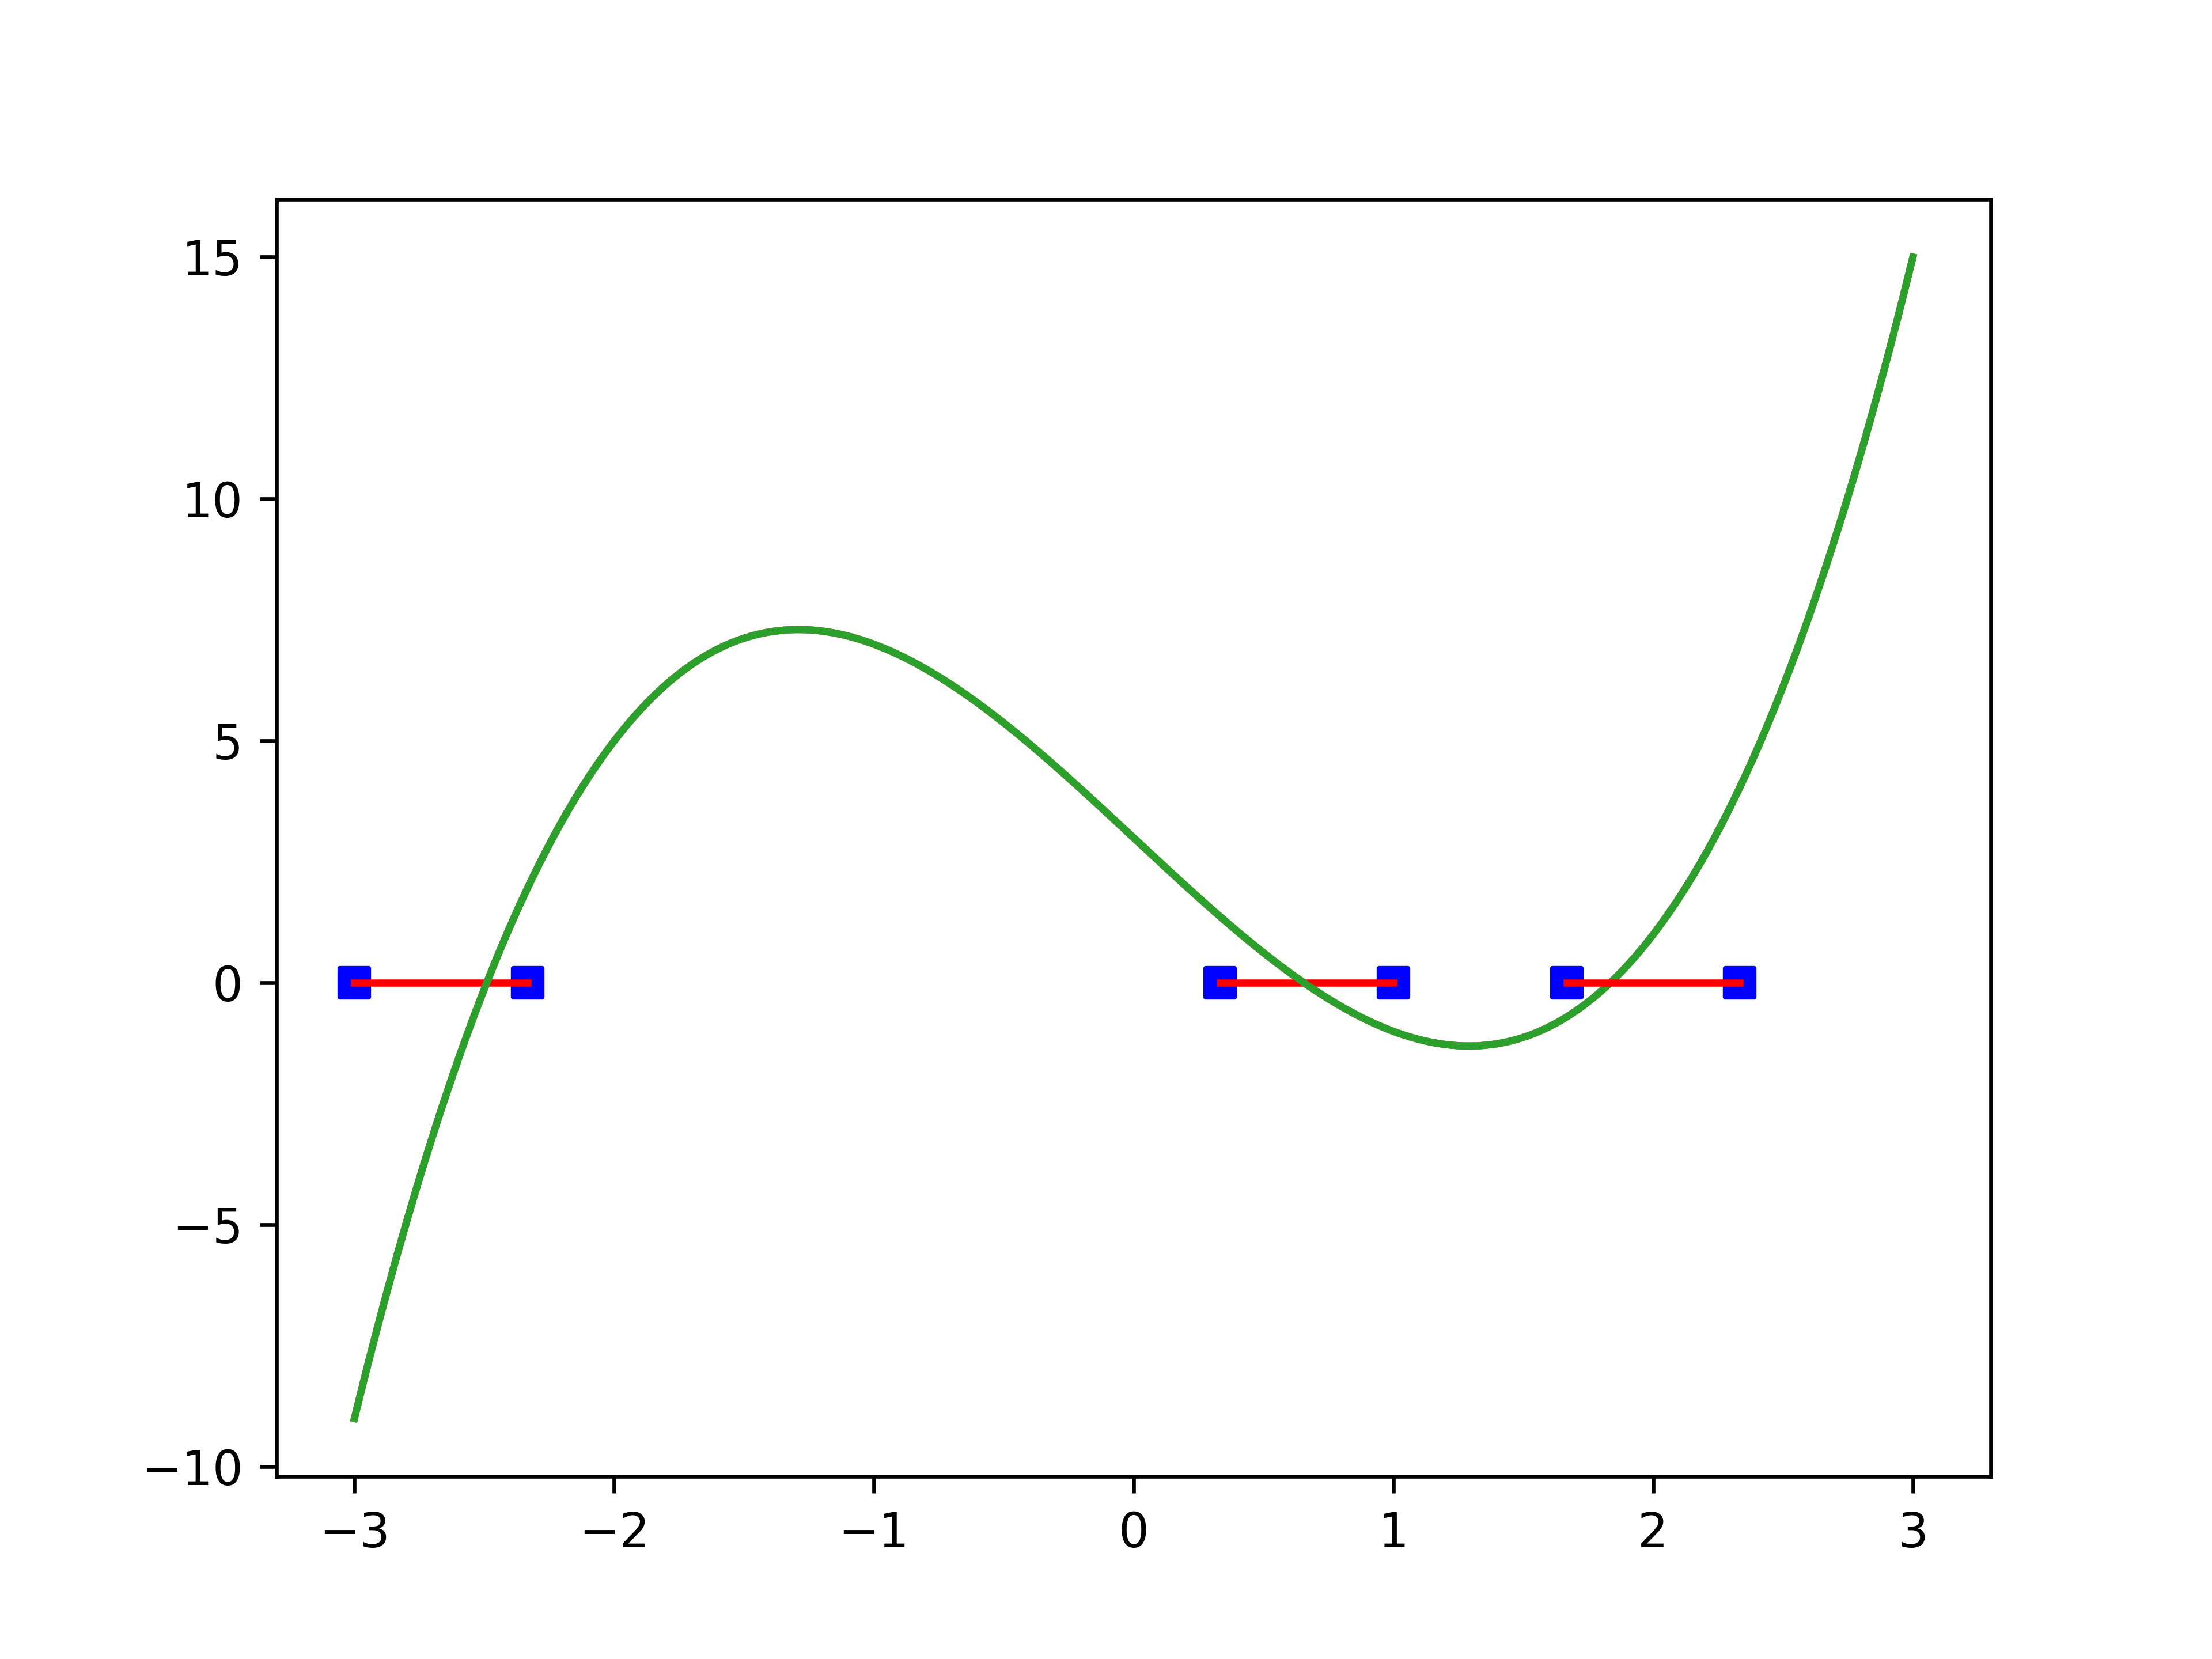
\includegraphics[width=1\linewidth]{photo/f(x) with bracket.png}
    \caption{f(x)-x图像。其中标出了由$find_bracket$函数找出的变号区域}
    \label{fig:1}
\end{figure}

\subsection{程序描述}
对于题目要求求解的方程,我们首先通过在一定范围内均匀采样(一般采样10个点)找到其变号区间,在程序中由$find\_bracket$完成(见图\ref{fig:1})。对于1.1题,我们使用$bisection\_method$函数接收其变号区间,并在区间内使用二分法逼近其中的根,直到误差在容差$10^(-4)$以下,这里根的误差使用二分区间大小$|a-b|$估计。对于1.2和1.3题,由于np.float64类型浮点数的精度大约只有16位有效位数左右,因此我们使用decimal库实现50位有效数字的计算。我们在$newton_raphson_method$和$hybrid_method$函数中接收由1.1中得到的解,将其误差缩小至$10^(-14)$以下,这里误差我们使用$|f(x)/f'(x)|$估计。

本程序源文件为WheatstoneBridge.py,在终端进入当前目录,使用命令
\Colorbox{cmdbg}{\lstinline[language=bash]|python -u WheatstoneBridge.py|}
运行本程序。运行时请保证此程序与题目一SketchFunction.py在同一文件夹下,且Python第三方库Numpy已安装。程序开发环境为Python3.9.6,可在Python3.8以上版本中运行。

\subsection{伪代码}
高斯消去法的伪代码如下所示
\begin{breakablealgorithm}
    \caption{Gaussian Elimination Method}
    \begin{algorithmic}[1]
        \Require $R$: Matrix(float, shape=(n, n+1))
        \Ensure $i$: Array(float, len=n)
        \For{$i \gets 1$ \textbf{to} $n$}
        \State $m \gets$ the index of $max(abs(R[i:n, i]))$\Comment(Pivot the matrix)
        \State swap row $i$ and row $m$ of the $R$
        \State $R_i \gets R_i / R_{ii}$ \Comment(Let the first element in this line equals 1)
        \For{$j \gets i+1$ \textbf{to} $n$}
        \State $R_j \gets R_j-R_i*R_{ji}$ \Comment(Produce the upper triangular matrix)
        \EndFor
        \EndFor
        \For{$i \gets n$ \textbf{to} $1$}
        \For{$j \gets 1$ \textbf{to} $i$}
        \State $R_j \gets R_j-R_i*R_{ji}$ \Comment(Produce the diagonal matrix)
        \EndFor
        \EndFor
        \State $i \gets$ the last column of $R$
        \State \Return $i$
    \end{algorithmic}
\end{breakablealgorithm}

\subsection{输入输出实例}
对于本程序,首先需要用户输入电路中六个电阻$(r_s,r_a,r_x,r_1,r_2,r_3)$的数值,通过这些电阻值写出增广矩阵$\boldsymbol{R}|\boldsymbol{v}$,将该增广矩阵带入高斯消去法中即可求得电流$\boldsymbol{i}$,等效电阻$r_e=v_0/i_1$。下列表格为在相应输入电阻下的运算结果

\begin{table}[ht!]
    \begin{center}
        \begin{tabular}{|c|c|c|c|c|c|c|c|}\hline
             & \multicolumn{6}{|c|}{Input} & \multicolumn{1}{|c|}{Output}\\\hline
            Index & $r_s$ & $r_a$ & $r_x$ & $r_1$ & $r_2$ & $r_3$ & $r_e$\\\hline
            \ding{172} & $4$ & $0$ & $5$ & $5$ & $7$ & $7$ & $10.00$\\\hline
            \ding{173} & $4$ & $100$ & $5$ & $5$ & $7$ & $7$ & $10.00$\\\hline
            \ding{174} & $1$ & $100$ & $5$ & $5$ & $7$ & $7$ & $7.00$\\\hline
            \ding{175} & $4$ & $100$ & $3$ & $5$ & $7$ & $2$ & $7.53$\\\hline
            \ding{176} & $4$ & $0$ & $3$ & $5$ & $7$ & $2$ & $7.43$\\\hline
        \end{tabular}
        \caption{问题二的结果实例}
    \end{center}
\end{table}

对比表格\ding{172}与\ding{173}可以看出,在电桥平衡的情况下,改变电流计阻值$r_a$并不会影响电路整体的等效电阻;对比表格\ding{173}与\ding{174}可以看出,电源内阻$r_s$的大小会直接影响电路电阻大小,$r_s$的变化量就是$r_e$的变化量,从物理上看这也是显然的;对比表格\ding{175}与\ding{176}可以看出,在电桥不平衡的情况下,改变电流计阻值会影响等效电阻$r_e$的大小,但在$r_a$变化较大的情况下,$r_e$变化仍较小。图\ref{fig:q2}是程序运行的实际截图。

\begin{figure}[ht]
    \centering
    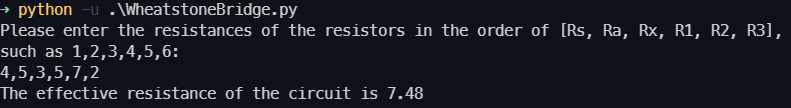
\includegraphics[width=0.9\linewidth]{photo/Q2.png}
    \caption{题目2 运行结果}
    \label{fig:q2}
\end{figure}


\end{document}
